\documentclass{standalone}
\usepackage{tikz}
\usepackage{ctex,siunitx}
\usepackage{tkz-euclide}
\usepackage{amsmath}
\usetikzlibrary{patterns,calc}
\usetikzlibrary {decorations.pathmorphing, decorations.pathreplacing, decorations.shapes,}
\begin{document}
\small
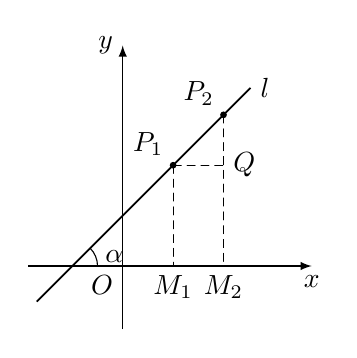
\begin{tikzpicture}[>=latex,scale=0.8]
  \draw[thin,->](-1.5,0)--(3.0,0)node[below]{$x$};
  \draw[thin,->](0,-1.0)--(0,3.5)node[left]{$y$};
  \draw[semithick](-0.8,0)--++(45:4.0)node[right]{$l$};
  \tkzDefPoints{0/0/O,1.6/2.4/P2,0.8/1.6/P1,0.8/0/M1,1.6/0/M2,1.6/1.6/Q}
  \tkzLabelPoints[below left](O)
  \tkzLabelPoints[right](Q)
  \tkzLabelPoint[above left](P1){$P_1$}
  \tkzLabelPoint[above left](P2){$P_2$}
  \tkzLabelPoint[below](M1){$M_1$}
  \tkzLabelPoint[below](M2){$M_2$}
  \tkzDrawSegments[densely dashed](P1,M1 P2,M2 P1,Q)
  \tkzDrawPoints[fill=black](P1,P2)
  \draw[semithick](-0.8,0)--++(-135:0.8);
  \draw(-0.4,0)arc(0:45:0.4)node[midway,right]{$\alpha$};
\end{tikzpicture}
\end{document}